\section{Dynamic Time Warping (DTW)}
Another commonly used metrics 
\footnote{It should be noted, that while a distance function is required to satisfy \ref{eq:d1} - \ref{eq:d4}, the Dynamic Time Warping (DTW) distance fails to satisfy the triangular inequality \ref{eq:d4} as shown in \cite{citeulike:4343286} and \cite{citeulike:4343933}.}
in time-series similarity is based on the Dynamic Time Warping algorithm (DTW). The DTW algorithm is a well-known algorithm in many areas. While first introduced in 60s \cite{citeulike:3733907} and extensively explored in 70s by application to the speech recognition \cite{citeulike:603020}, \cite{citeulike:3496861} it is currently used in many areas: handwriting and online signature matching \cite{citeulike:2838910} \cite{citeulike:2584345}, sign language recognition \cite{citeulike:3789957} and gestures recognition \cite{citeulike:3789964} \cite{citeulike:3789957}, data mining and time series clustering (time series databases search) \cite{citeulike:3815076} \cite{citeulike:3733893} \cite{citeulike:3788783} \cite{citeulike:3731715} \cite{citeulike:3731713} \cite{citeulike:3789897}, computer vision and computer animation \cite{citeulike:3728229}, surveillance \cite{citeulike:964832}, protein sequence alignment and chemical engineering \cite{citeulike:3733894}, music and signal processing \cite{citeulike:3736775} \cite{citeulike:3728229} \cite{citeulike:3728228}.

The idea behind the DTW algorithm lies in allowing shifts of the data points in time and relies on the usage of Dynamic Programming \cite{citeulike:3733907} for optimal time-series alignment. Algorithm starts by building the distance matrix $C \in \mathbb{R}^{N \times M}$ representing all pairwise distances between $X$ and $Y$. This distance matrix called the \textbf{local cost matrix} for the alignment of two sequences $X$ and $Y$:
\begin{equation}
\label{eq:localcost}
C_{l} \in \mathbb{R}^{N \times M} \; : \; c_{i,j} = \left\| x_{i} - y_{j} \right\|, \; i \in [1:N], \; j \in [1:M]
\end{equation}
Once the local cost matrix built, the algorithm finds the \textbf{alignment path} which runs through the low-cost areas - ``valleys'' on the cost matrix, Figure \ref{fig:dtw}. This alignment path (or \textbf{warping path}, or \textbf{warping function}) defines the correspondence of an element $x_{i} \; \in \; X$ to $y_{j} \; \in \; Y$ following the boundary condition which assigns first and last elements of $X$ and $Y$ to each other, Figure \ref{fig:dtw}.

\begin{figure}[tbp]
   \centering
   \includegraphics[height=60mm]{dtw.eps}
   %%{seriesheatmap}
   \caption{Illustration of the DTW algorithm. Left: the raw time-series; center: the alignment matrix and the optimal alignment path; right: aligned time-series.}
   \label{fig:dtw}
\end{figure} 

Formally speaking, the alignment path built by DTW is a sequence of points $p=(p_{1}, p_{2}, ... , p_{K})$ with $p_{l} = (p_{i}, p_{j}) \in [1:N] \times [1:M]$ for $l \in [1:K]$ which must satisfy to the following criteria:
\begin{enumerate}
	\item \textbf{Boundary condition}: $p_{1}=(1,1)$ and $p_{K}=(N,M)$. The starting and ending points of the warping path must be the first and the last points of aligned sequences.
	\item \textbf{Monotonicity condition}: $n_{1} \leq n_{2} \leq ... \leq n_{K}$ and $m_{1} \leq m_{2} \leq ... \leq m_{K}$. This condition preserves the time-ordering of points.
	\item \textbf{Step size condition (continuity)}: this criteria limits the warping path from long jumps (shifts in time) while aligning sequences. While this condition significantly impacts performance of the algorithm and was explored in many works, the basic step size condition formulated as $p_{l+1}-p_{l} \in \left\{ (1,1), (1,0), (0,1) \right\}$.
\end{enumerate}

The \textbf{cost function} associated with a warping path computed with respect to the local cost matrix (which represents all pairwise distances) will be: 

\begin{equation}
\label{eq:pathcost}
c_{p}(X,Y) = \sum_{l=1}^{L} c(x_{n_{l}}, y_{m_{l}})
\end{equation}

The warping path which has a minimal cost associated with alignment called the \textbf{optimal warping path} $P^{*}$. Once computed, it used for time-series alignment, Figure \ref{fig:dtw}.

It's quite interesting that Euclidean distance is the special case of the DTW distance with applied restriction that $i=j=k$.

The time and space complexity of the DTW distance is $O(nm)$
